\documentclass[border=10pt]{standalone}
\usepackage{xcolor}
\usepackage{tikz}
\usetikzlibrary{arrows.meta,positioning,fit,backgrounds}

\definecolor{BG}{HTML}{FAFAFA}
\definecolor{INK}{HTML}{1A1A2E}
\definecolor{SUB}{HTML}{555566}
\definecolor{COLD}{HTML}{4361EE}
\definecolor{WARM}{HTML}{2EC4B6}
\definecolor{JOB}{HTML}{D81159}
\definecolor{MIR}{HTML}{9B5DE5}

\begin{document}
\pagecolor{BG}
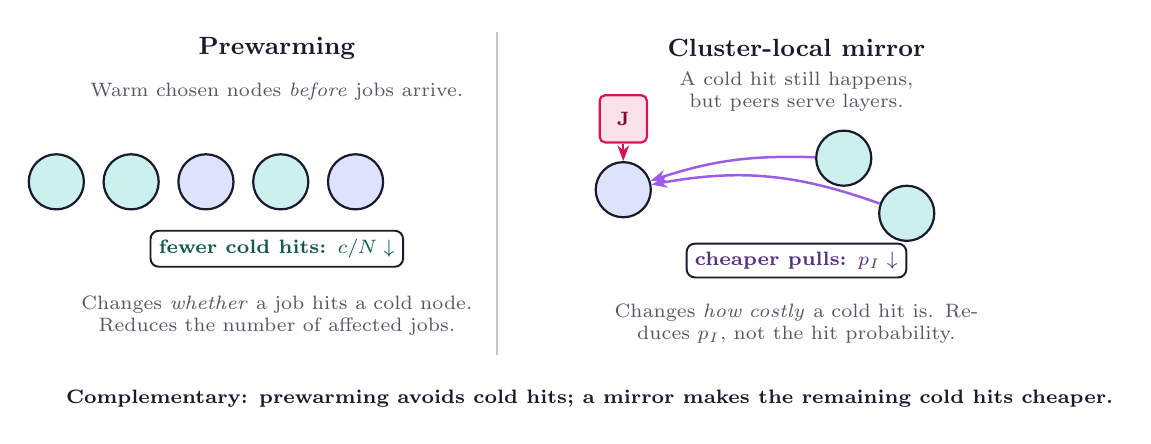
\begin{tikzpicture}[
  font=\sffamily,
  nd/.style={circle, draw=INK, line width=0.8pt, minimum size=7mm, inner sep=0pt},
  cold/.style={nd, fill=COLD!18},
  warm/.style={nd, fill=WARM!25},
  head/.style={font=\small\bfseries, text=INK},
  note/.style={font=\scriptsize, text=SUB, align=center},
  tag/.style={rounded corners=3pt, draw=INK, line width=0.7pt, fill=white, font=\scriptsize\bfseries, inner sep=3pt},
]

% ===== LEFT: prewarming =====
\node[head] at (2.8, 3.3) {Prewarming};
\node[note, text width=5.2cm] at (2.8, 2.75)
  {Warm chosen nodes \emph{before} jobs arrive.};
\foreach \i/\s in {0/warm,1/warm,2/cold,3/warm,4/cold} {
  \node[\s] (p\i) at (\i*0.95, 1.6) {};
}
\node[tag, text=WARM!45!black] at (2.8, 0.75) {fewer cold hits: \(c/N \downarrow\)};
\node[note, text width=5.4cm] at (2.8, -0.1)
  {Changes \emph{whether} a job hits a cold node. Reduces the number of affected jobs.};

% divider
\draw[SUB!35, line width=0.6pt] (5.6, -0.6) -- (5.6, 3.5);

% ===== RIGHT: mirror =====
\begin{scope}[xshift=6.6cm]
\node[head] at (2.8, 3.3) {Cluster-local mirror};
\node[note, text width=5.4cm] at (2.8, 2.75)
  {A cold hit still happens, but peers serve layers.};
\node[cold] (m0) at (0.6, 1.5) {};
\node[rounded corners=2pt, fill=JOB!12, draw=JOB, line width=0.8pt, minimum size=6mm, inner sep=1pt, font=\scriptsize\bfseries, text=JOB!60!black] (mj) at (0.6, 2.4) {J};
\draw[-{Stealth[length=2mm]}, JOB, line width=0.7pt] (mj) -- (m0);
\node[warm] (mp1) at (3.4, 1.9) {};
\node[warm] (mp2) at (4.2, 1.2) {};
\draw[-{Stealth[length=2mm]}, MIR, line width=0.9pt] (mp1) to[bend right=10] (m0);
\draw[-{Stealth[length=2mm]}, MIR, line width=0.9pt] (mp2) to[bend right=15] (m0);
\node[tag, text=MIR!55!black] at (2.8, 0.6) {cheaper pulls: \(p_I \downarrow\)};
\node[note, text width=5.4cm] at (2.8, -0.2)
  {Changes \emph{how costly} a cold hit is. Reduces \(p_I\), not the hit probability.};
\end{scope}

\node[font=\scriptsize\bfseries, text=INK, anchor=west] at (0.0, -1.15)
  {Complementary: prewarming avoids cold hits; a mirror makes the remaining cold hits cheaper.};

\end{tikzpicture}
\end{document}
